% Chapter 4

\chapter{Dataset creation}
\label{Chapter4}

In Chapter~\ref{Chapter3} we finalised our OpenAI environment choice and have a systematic way to generate different configurations of our environments.

The next step is to build up our dataset by solving as many of these configurations as possible with the use of reinforcement learning algorithms.

We justified in previous sections (specifically section~\ref{qlearning} and section~\ref{movationandshortcomings}) how using \emph{model-free} reinforcement learning algorithms will put us in the right direction to achieve the project's goals highlighted in section~\ref{motivation}: improve the transferability of pre-trained models to different configurations, environments, and tasks.

One choice that is left to make before we move on to train models using our randomised environments is what reinforcement learning algorithm we should use.

%----------------------------------------------------------------------------------------

\section{Q-learning on \code{RandomisedFrozenLake}}
We have presented Q-learning in section~\ref{qlearning} as a method that generates a policy by building up a table $Q$ of values corresponding to the expected utility of taking each action at each observable state.

This table $Q$ is represented as a 2D-matrix of size (\code{env.observation\_space.n}, \code{env.action\_space.n}), which in the case of \code{RandomisedFrozenLake} is just a (16x4) matrix.

This is good news. Having a policy that is encoded as a 2-dimensional data structure makes it an obvious input to our Generative Adversarial Network later on in the next chapter. In fact, as we presented in section~\ref{successes}, GANs have proven successful in image synthesis applications, where inputs were images, that is 2D matrices.

The choice of Q-learning as our reinforcement learning technique therefore becomes preferable. Other model-free algorithms like policy search may not have a clear 2D representation in the way the trained parameter set $\theta$ is encoded.

%----------------------------------------------------------------------------------------

\section{Experiment set up}
Before we proceed, we need to be able to record some details about the process of training our data. If our ultimate objective is to benchmark performance of traditional reinforcement learning agains our proposed approach, we need to record running time of our training, and see if that improves at the end. 

Let's encapsulate training of a configuration in an \code{Experiment} class, whose code is shown in listing~\ref{lst:experiment}. An \code{Experiment} is initialised with an OpenAI Gym environment, which in our case is an instance of a \code{RandomisedFrozenLake}, and an integer value \code{num\_episodes}, indicating the number of independent simulations the Q-learning algorithm will be doing. By calling \code{Experiment}'s \code{run()} instance method, we actually start training the model, with $Q$ being updated at each iteration.

The instance variable \code{score} could be used as an evaluation criteria of the effectiveness of our training. It records the average reward the agent achieves for each episode during training.

\code{Experiment} also has a utility method called \code{dumps()} that serialises all this data and allows us to save it on disk.
\\\\
\begin{minipage}{\linewidth}
\lstset{language=Python}
\lstset{frame=lines}
\lstset{caption={\code{Experiment} wrapper class to train one instance of \code{RandomisedFrozenLake}}}
\lstset{label={lst:experiment}}
\lstset{basicstyle=\footnotesize}
\begin{lstlisting}
class Experiment(object):
    def __init__(self, env, num_episodes=10000):
        self.env = env
        self.Q = np.zeros([self.env.observation_space.n, self.env.action_space.n])
        self.num_episodes = num_episodes
        self.score = None
        self.valid_score = None
        self.start = None
        self.end = None
            
    def run(self):
        self.start = datetime.now()
        # ------------------------------------------------------------
        # Run Q-learning algorithm, saving the rewards of each episode
        # ...
        # ...
        # ------------------------------------------------------------
        self.end = datetime.now()
        self.score = sum(rewards)/self.num_episodes
        
    def dumps(self):
        return dumps({'Q': self.Q, 'start': self.start, 'end': self.end, 'score': self.score, 'num_episodes': self.num_episodes})
\end{lstlisting}
\end{minipage}

It's critical to be able to evaluate the quality of the Q-table after training. To do so we just use the optimal policy (that is the policy that picks the action that has the maximum expected utility according to the Q-table) and run if for a certain number of episodes. A validation score could be then defined by the average reward achieved at each episode. Listing \ref{lst:validate_experiment} shows the code to achieve that.

\begin{minipage}{\linewidth}
\lstset{language=Python}
\lstset{frame=lines}
\lstset{caption={Code to validate a trained Q-table}}
\lstset{label={lst:validate_experiment}}
\lstset{basicstyle=\footnotesize}
\begin{lstlisting}
def validate(self):
	rewards = 0
    for i in tqdm(range(num_episodes)):
        while j < 200: # Limit to 200 time steps
            j+=1
            # Choose an action by pick best action from Q-table
            a = np.argmax(Q[s,:])
            
            # Get new state and reward from environment
            s1,r,d,_ = env.step(a)
            rewards += r
            s = s1
            if d == True:
                break
     self.valid_score = rewards / num_episodes
\end{lstlisting}
\end{minipage}

%----------------------------------------------------------------------------------------

\section{Distributed Q-learning}
Now that we formalised our experiment setup, we can run Q-learning on each of the map configurations of our \code{RandomisedFrozenLake}. For the 4x4 grid there are 3827 possible valid map configurations. It takes an average of 15 seconds to train each Q-learning table on a 2.5 GHz Intel Core i7 processor. On a single machine, it would take around 16 hours to run each experiment.

To make this step of our pipeline faster and scalable to more data, we decide to set up a distributed processing on a cluster with multiple machines. More precisely, we set up a MapReduce framework \parencite{Dean:2004:MSD:1251254.1251264} implementation running on a Hadoop cluster \parencite{shvachko2010hadoop}.

A MapReduce program is composed of a Map procedure that takes in some (large) input and performs a particular operation whose output is then fed into another Reduce procedure, which outputs the final result. The power of MapReduce is that the framework orchestrates the processing of these procedures by marshalling the distributed servers, running the various tasks in parallel, managing all communications and data transfers between the various parts of the system, and providing for redundancy and fault tolerance.

Figure~\ref{fig:MapReduce} shows the distributed architecture to train multiple Q-learning instances. The input to the system is a list of strings, each representing the map configuration of a \code{RandomisedFrozenLake}, e.g. $"SFHHHFHHHFHHHFFG"$. These inputs are fed into Mapper programs running on different machines. The mapper's task is to initialise the experiment and run Q-learning on the environment. It outputs a key-value pair, where the key is the string that uniquely identifies a map configuration, and the output is the \code{Experiment} object that encapsulates the already trained Q-table. We have yet to assign a validation score to this table we trained, and that's the job of the reducer.

Each experiment's result is then written on an output file by the reducer. Each line will be again a key-value pair, with the map configuration string as key and the \code{Experiment} result dumped in string format. In our following sections, we can just parsing and load these results to conduct our further analysis.

While this particular architecture does not make full use of the power of MapReduce (combining, partitioning and sorting), it is an optimal and convenient pipeline to distribute our computations across a cluster of machines, thereby drastically reducing our training time.
\begin{figure}
\centering
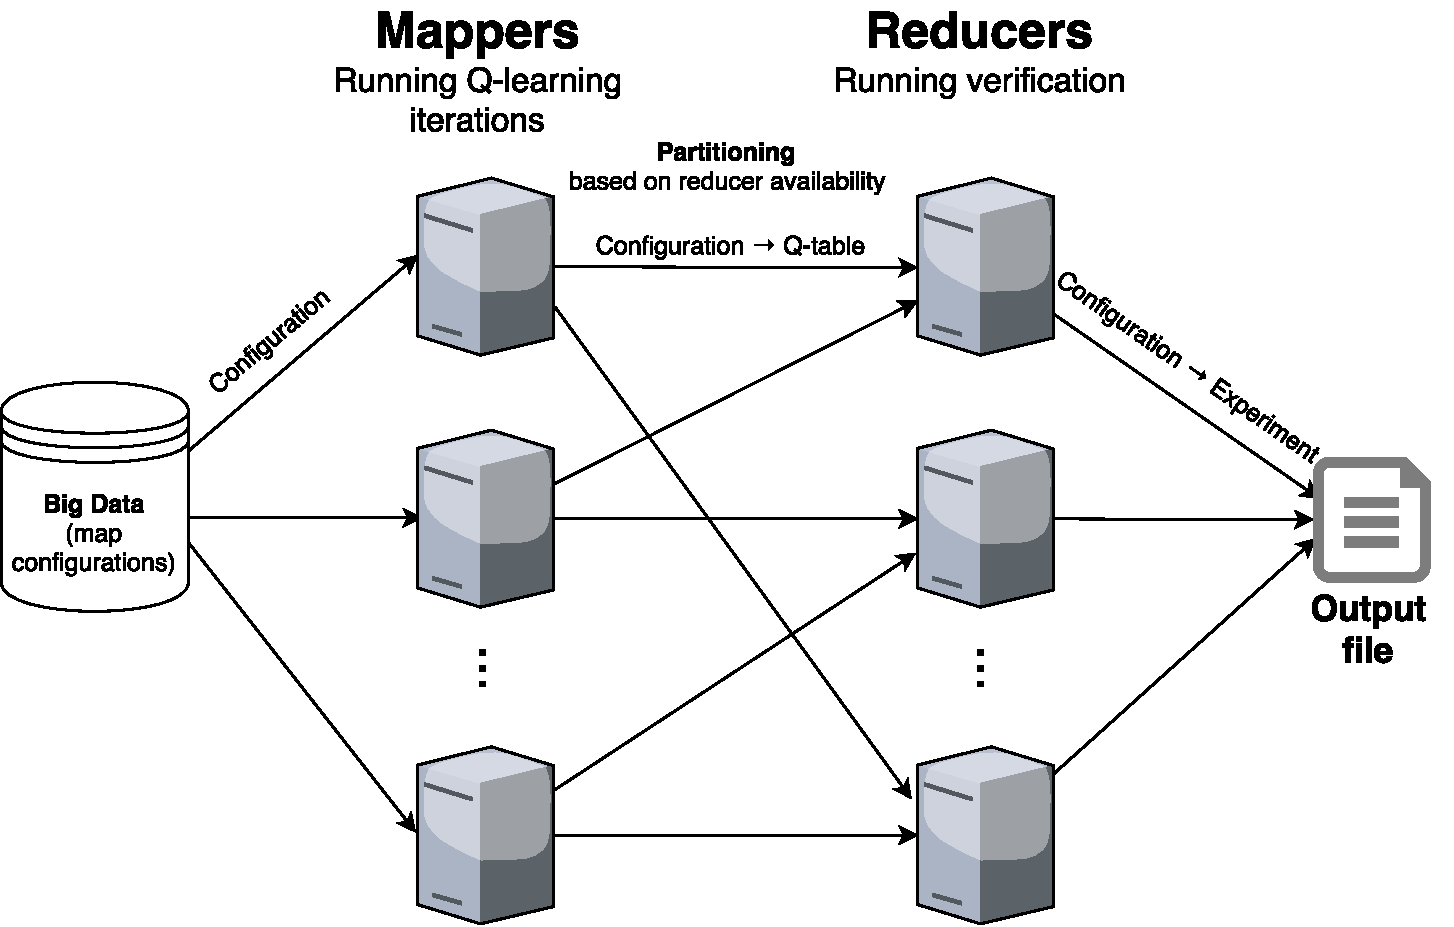
\includegraphics[width=10cm]{Figures/MapReduce}
\caption{Schematic of distributed Q-learning with validation on MapReduce}
\label{fig:MapReduce}
\end{figure}

%----------------------------------------------------------------------------------------